\documentclass[12pt,a4paper]{article}
\synctex=1
\usepackage[utf8]{inputenc}
\usepackage[margin=1cm]{geometry}
\usepackage{graphicx}
%\usepackage{verbatim}
\usepackage{amsmath}
\usepackage{amsfonts}
\usepackage{amssymb}
\usepackage{listings}
\usepackage{enumitem}
\usepackage{textcomp}
\usepackage{courier}
\usepackage{libertine}
\usepackage{pgfornament}
\usepackage{eso-pic}
\usepackage[hangul]{kotex}
\linespread{1.3}

\title{
	\centering
	\pgfornament[width=12cm,color=teal]{84}\\
	\vspace{1cm}
	\fontsize{50}{50} \selectfont {정보통신 수학 및 실습\\Lab assignment}\\
		\pgfornament[width=12cm,color=teal]{88}\\
	\vfill}
\author{
	\LARGE
	\begin{tabular}{rcc}
		\hline
		학번 : & 2016110056 & 2012112130\\ 
		이름 : & 박승원 & 노희승\\
		편성 : & 20조 & \today\\
		\hline
	\end{tabular}\vspace{1cm}
	\\
\includegraphics[width=0.5\textwidth]{logo.jpg}
	}
\date{}

\begin{document}
\maketitle
\pagenumbering{gobble}
\noindent
\lstset{language=matlab, columns=flexible, tabsize=4, frame=shadowbox, showstringspaces=false, breaklines=true, upquote=true, basicstyle=\normalsize}

\renewcommand{\thesubsubsection}{\alph{subsubsection})}
\renewcommand{\thesubsection}{\arabic{subsection}.}
\newpage
\section*{Chapter 3. Lab Assignment}
\subsection{Plot the following cosine functions using MATLAB and write down their frequencies.  You must define the boundaries and the intervals of variable t properly to obtain at least one cycle of the function.  [Hint: use t such that $wt > 2\pi\times n$, where n is the number of cycles in the plot.]} 

\subsubsection{$\cos(5t)$}
$2\pi f = 5\\
\therefore f = \dfrac{5}{2\pi}$

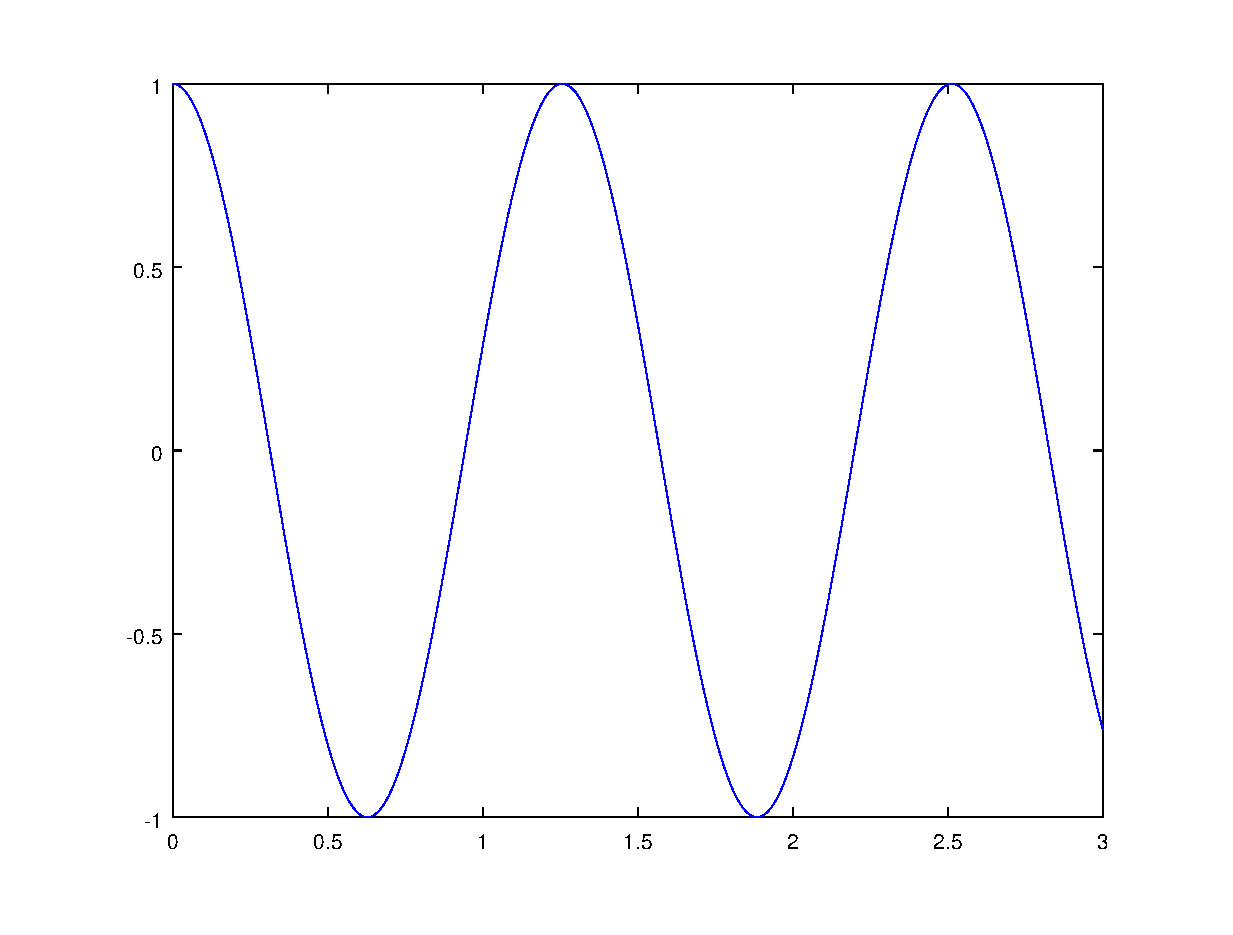
\includegraphics[width=0.8\textwidth]{a.eps}

\subsubsection{$\cos(2\pi 100t)$}
$2\pi f = 2\pi 100\\
\therefore f = 100$

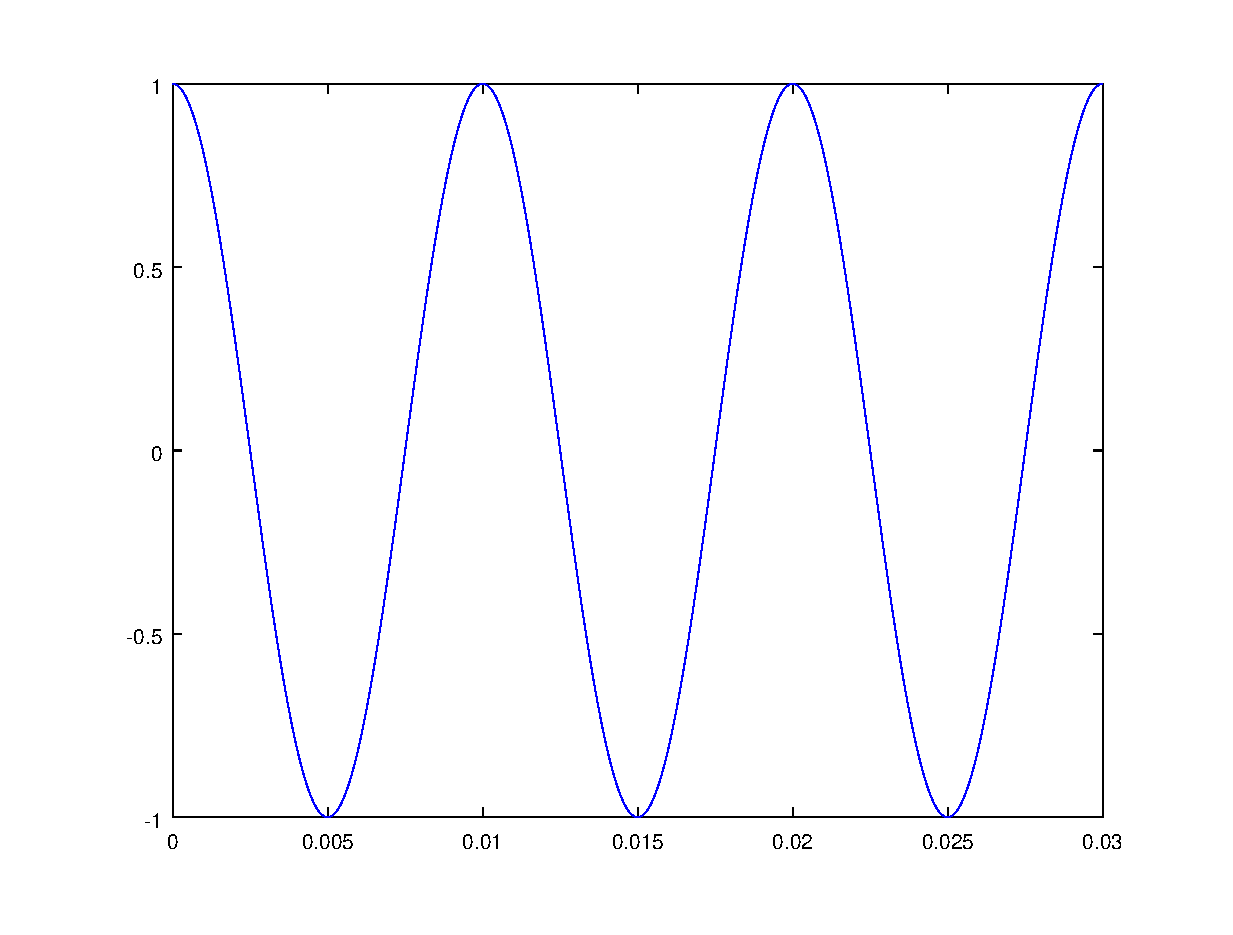
\includegraphics[width=0.8\textwidth]{b.eps}

\subsection{If the sound signal is defined as $m(t)=\cos(2\pi(10)t)$ and the carrier signals is $\cos(2\pi (300)t)$, answer the following questions: (Hint: use t=[0:0.0001:1])} 

\begin{lstlisting}
>> t = [0:0.0001:1];
>> ct = cos(2*pi*200*t);
>> mt = cos(2*pi*10*t);
>> plot(t(1:3000),mt(1:3000))
>> print -depsc 2a.eps
>> plot(t(1:3000),ct(1:3000))
>> print -depsc 2b.eps
>> xc = mt.*ct;
>> plot(t(1:3000),xc(1:3000))
\end{lstlisting}

\subsubsection{Plot mt(1:3000)}
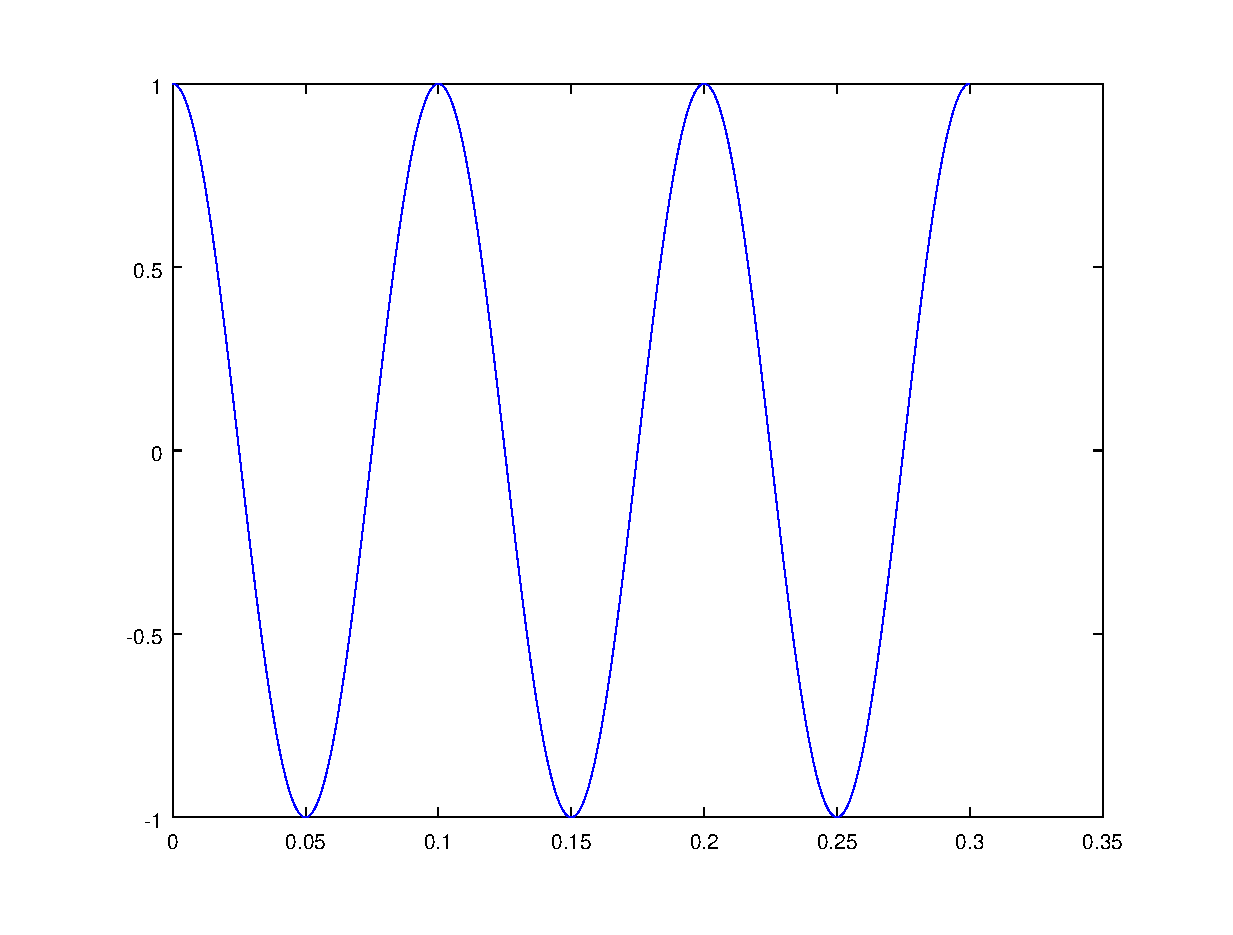
\includegraphics[width=0.8\textwidth]{2a.eps}
\subsubsection{Plot ct(1:3000)}
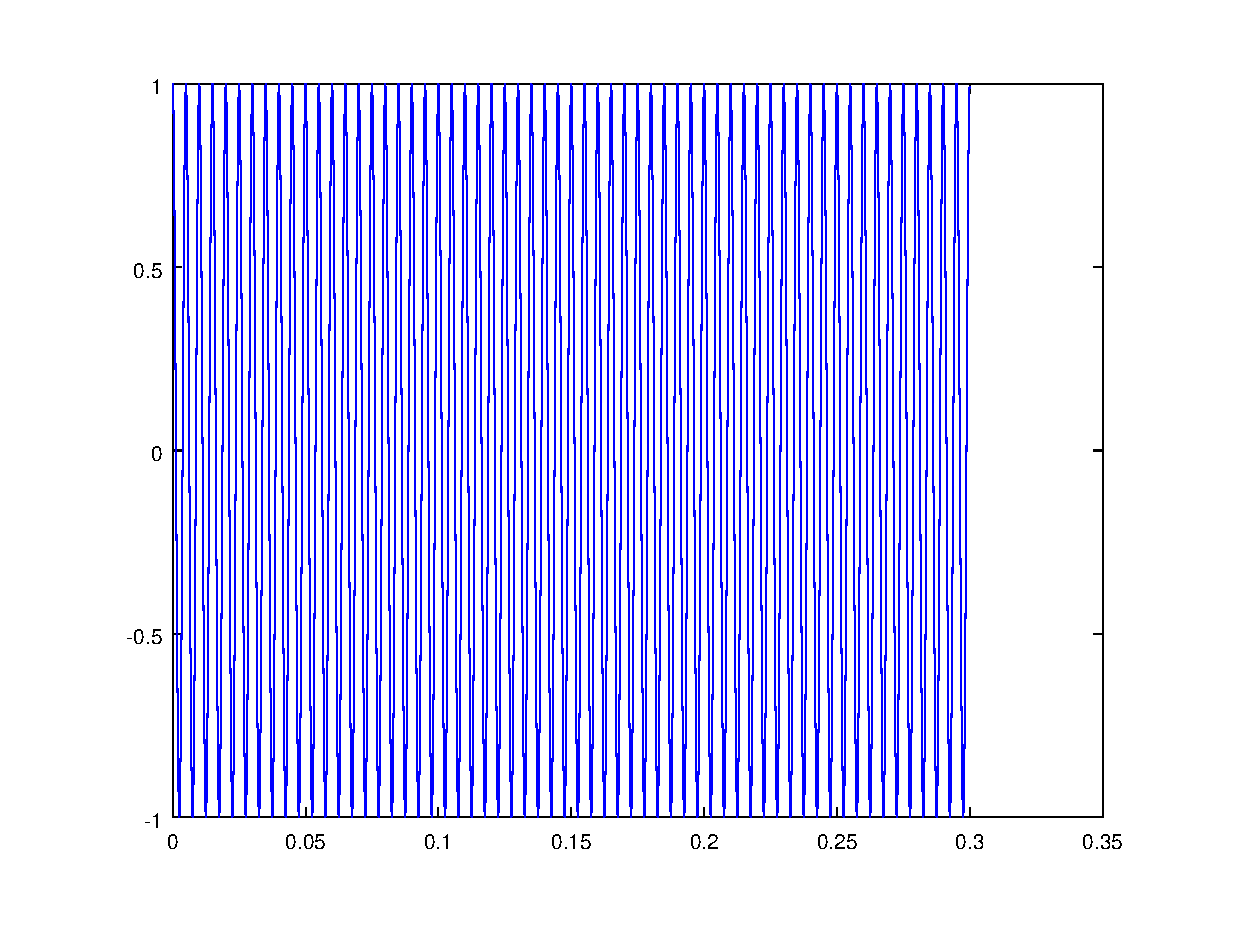
\includegraphics[width=0.8\textwidth]{2b.eps}
\subsubsection{Plot xc = mt * ct for xc(1:3000)}
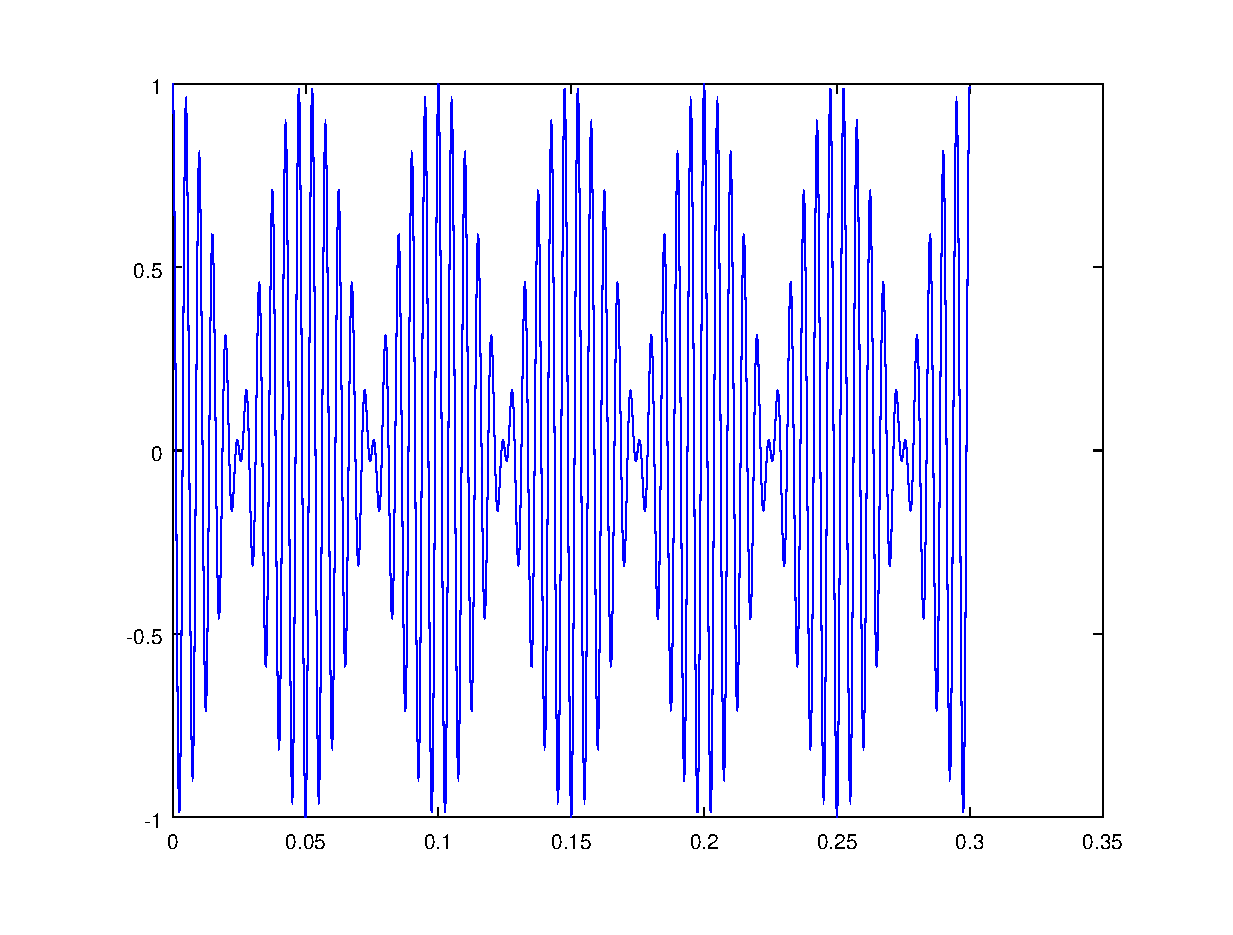
\includegraphics[width=0.8\textwidth]{2c.eps}

\subsubsection{Plot the spectrum of signal xc using the following commands:\\spec=abs(fft(xc));\\N=length(spec)/2;\\plot(spec(1:700)/N)}

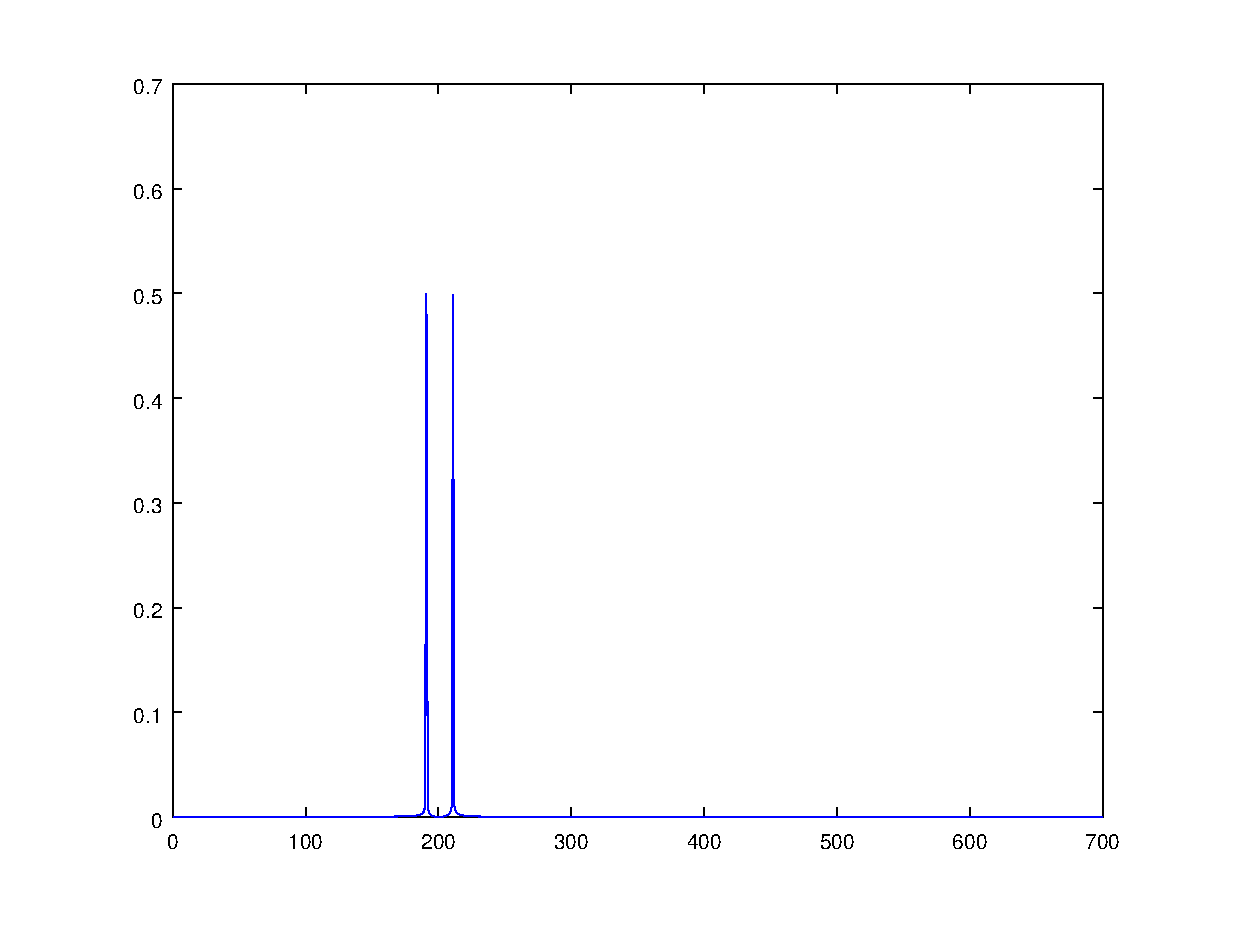
\includegraphics[width=0.8\textwidth]{2d.eps}

\subsubsection{Plot xi=xc*ct for xi(1:3000).}
\begin{lstlisting}
>> xi = xc .* ct;
>> plot(t(1:3000), xi(1:3000))
\end{lstlisting}

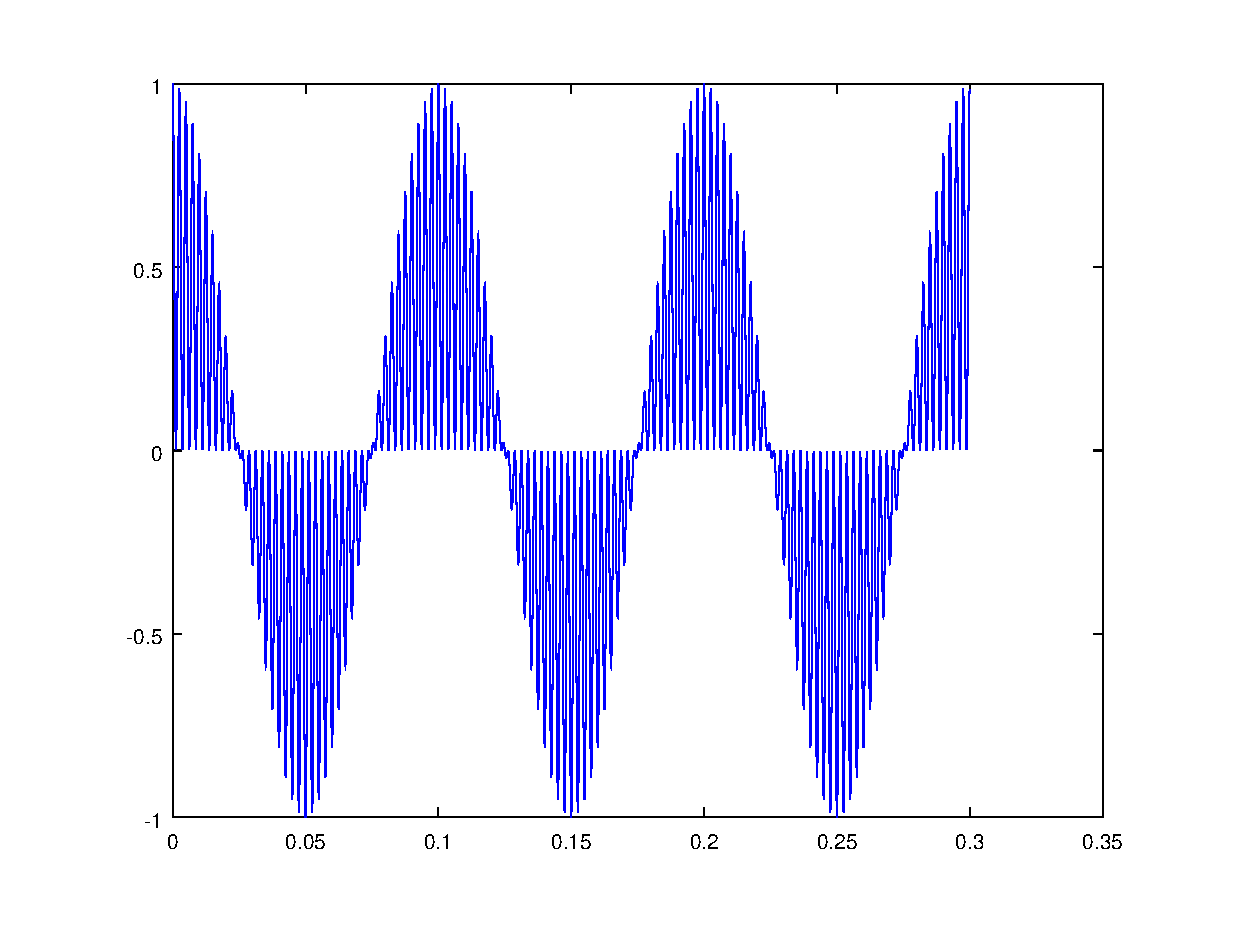
\includegraphics[width=0.8\textwidth]{2e.eps}
 
\subsubsection{Plot the spectrum of signal xi using the following commands:\\spec2=abs(fft(xi));\\N=length(spec2)/2;\\plot(spec2(1:700)/N)}          
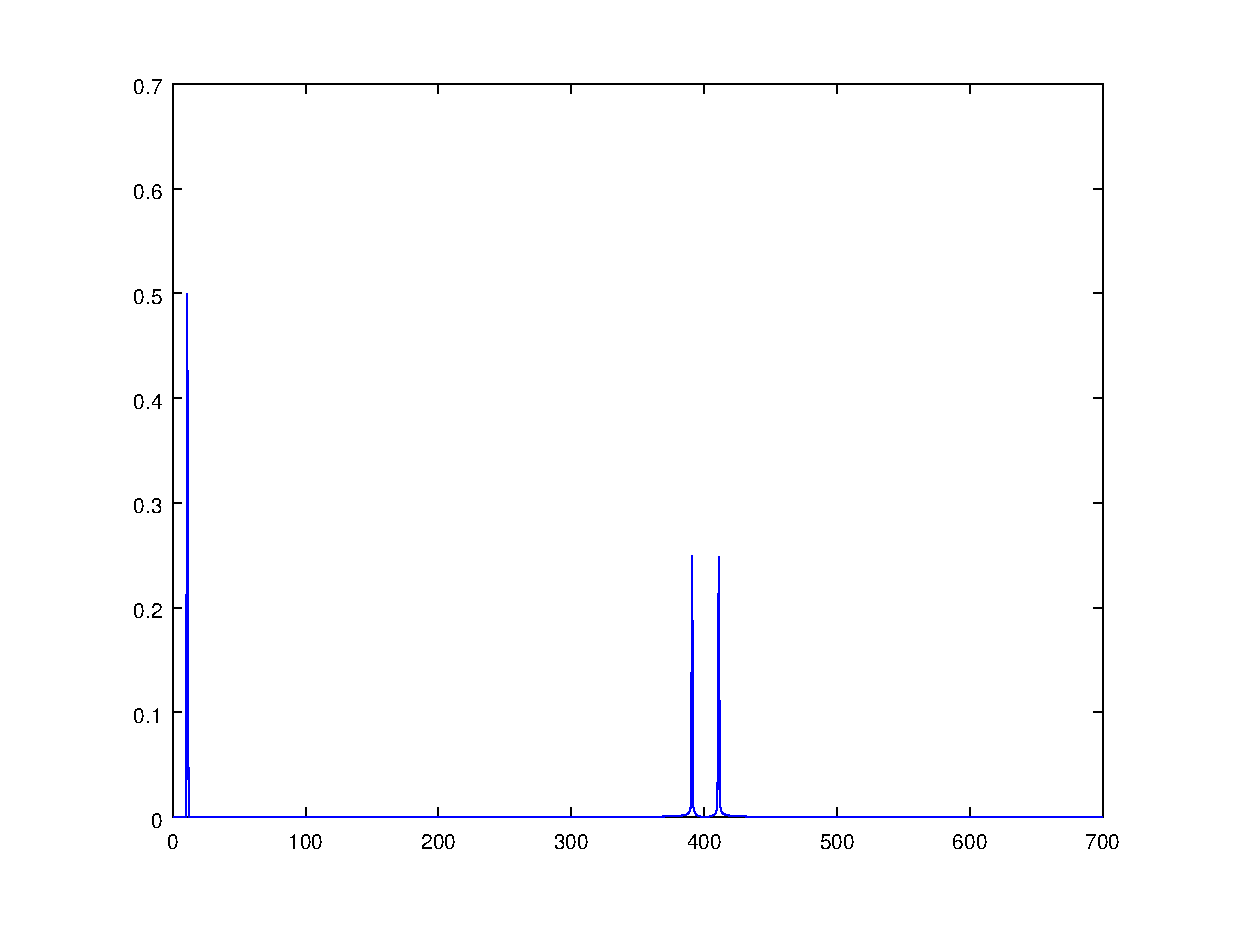
\includegraphics[width=0.8\textwidth]{2f.eps}

\subsubsection{What must be the cutoff frequency of LPF to recover mt from xi?} 
10보다 커야 한다.
\end{document}
